\documentclass[12pt,a4paper]{article}


\usepackage[utf8]{inputenc}
\usepackage[T2A]{fontenc}
\usepackage[russian]{babel}
\usepackage{amsfonts,amsmath,amssymb,longtable,hhline}
\usepackage{multicol}
\usepackage{color,soul}
\usepackage{booktabs, tabularx}
\usepackage{graphicx}
\usepackage{titlesec}
\usepackage{wrapfig}
\usepackage{float}


\hoffset=-1.5cm\voffset=-2cm \textwidth=17.1cm \textheight=23.0cm
\parindent=1.20cm 
\righthyphenmin=2     
\renewcommand*{\baselinestretch}{1.05} 
\tolerance=1000         


\renewcommand{\thefootnote}{}


\begin{document}
\large


\noindent УДК 004.94; 656.1; 519.8
\bigskip


\centerline{\bf \LARGE Перколяционный анализ транспортной сети }
\centerline{\bf \LARGE с выявлением критических дорог.}
\bigskip


\centerline{\bf © 2025 г. \ \ Е. С. Данович$^{1}$, \ \ В. А. Ивенин$^{1,*}$, \ \ О. О. Рыбалов$^{1}$, \ \ М. С. Титов$^{1}$}


\bigskip
\centerline{$^{1}$ Центральный университет, 123056, г. Москва, ул. Гашека, д. 7, стр. 1}
\centerline{$^{*}$\it email: iveninvala7@gmail.com} 

\bigskip

Данная работа посвящена применению теории перколяции для комплексного анализа устойчивости городских транспортных сетей к деградации инфраструктуры. 
Исследование проведено на примере сетей Москвы, Северного административного округа и Замоскворечья, 
смоделированных как ориентированные графы с реалистичными параметрами потоков. Методология основана на анализе двух сценариев деградации сети: 
случайном выведении элементов из строя и целенаправленной атаке на наиболее критичные рёбра. 
Исследование подтверждает необходимость учёта динамических характеристик транспортных потоков и фокусирования усилий на защите уязвимых элементов инфраструктуры. 
Полученные геопространственные визуализации позволяют локализовать наиболее критичные участки на карте города 
и прогнозировать распространение заторов при превышении порога перколяции. 

\medskip
\textit{Ключевые слова:} перколяция, транспортные сети, критические дороги, графовые модели, визуализация.
\medskip

\newpage
\begin{multicols}{2}


\section{Введение}\label{Introduction}


Транспортные сети представляют собой сложные инфраструктурные системы, подверженные постоянному риску сбоев, вызванных как естественными причинами 
(перегрузки в часы пик, дорожно-транспортные происшествия, перекрытия), так и чрезвычайными ситуациями 
(стихийные бедствия, отказы ключевых инфраструктурных элементов, таких как кольцевые развязки или тоннели). 
Определение наиболее критичных участков сети, таких как мосты или ключевые перекрестки, и прогнозирование момента, когда сбои в работе отдельных, 
даже территориально небольших, участков сети могут приводить к нелинейным, каскадным эффектам, 
вызывающим масштабные заторы и паралич транспортного сообщения на обширных территориях, является актуальной задачей. 
Так, 11 декабря 2025 года ввиду перекрытия нескольких улиц в центре Москвы по данным сервиса «Яндекс.Карты» движение встало: 
10-бальные пробки по всей Москве \cite{rbc2025}(рис.~\ref{fig:moscow_traffic}).

В качестве решения проблемы перегрузки центра, как на данном примере, 
было предложено перенести железнодорожные вокзалы за пределы МКАД \cite{gluharuv1995, gluharuv2013}. 
Такое решение уменьшило бы общий автомобильный трафик в пределах города, особенно в центральном транспортном узле, 
и позволило бы использовать освободившиеся территории для уменьшения плотности автомобилей, и с их помощью можно было бы избежать такой проблемы.

\begin{figure*}[!ht]
    \centering
    \includegraphics[width=0.6\textwidth]{./view/10red.png}
    \caption{Транспортная ситуация в Москве 11 декабря 2025 года по данным сервиса <<Яндекс.Карты>>}
    \label{fig:moscow_traffic}
\end{figure*}

Проблема определения критических элементов и порогов устойчивости транспортных сетей не является новой и активно исследуется в научной литературе 
с применением различных подходов, включая теорию сложных сетей и перколяционный анализ, возможность применения которого доказана в \cite{nekrasova2015}. 
В дальнейшем теория перколяции была успешно применена для нахождения усовершенствованного подхода к выявлению критических рёбер в транспортных сетях \cite{gasparyan2025, balamirzoev2019}. 
В последующих научных исследованиях ученые приходят к выводу, что для эффективного моделирования потоков, 
а также для нахождения наиболее критичных узлов сети целесообразно сначала провести глубокий структурный анализ всей сети, указав наиболее влиятельные компоненты, 
и только после этого выделять зону влияния каждого из них и рассматривать их отдельно друг от друга \cite{khabarov2024}. Изучение идеи учета динамики сети показывает, 
что простого топологического анализа недостаточно. Результаты исследования \cite{gasparyan2025} свидетельствуют о том, 
что учет пространственно-временной сети является важным условием для точного прогнозирования критических рёбер в реальном или конкретно заданном времени. 
Задача автоматизированного планирования сети лесных дорог была решена в \cite{pyatin2020, katarov2023} с использованием графовой математической модели, 
что позволяет применить данный метод для аналогичного рассмотрения транспортной сети в городе.


Несмотря на наличие значительного объема исследований, посвященных отдельным аспектам анализа транспортных систем, 
остается не до конца решенной задача комплексного применения теории перколяции для точного определения 
наступления момента потери связности транспортной сети в реальных городских сетях, 
подверженных отказам ключевых инфраструктурных элементов (мостов, перекрестков). Существующие работы часто фокусируются либо на абстрактных моделях, 
либо на качественной оценке критичности. В данной работе мы стремимся заполнить этот пробел. Целью нашего исследования является разработка 
и апробация количественной методологии, которая позволит не только точно определить критические дороги и мосты, оказывающие наибольшее влияние на пропускную способность системы, 
но и оценить порог перколяции - критическую долю отключенных дорог, при которой транспортная сеть необратимо теряет связность 
и перестает функционировать как единое целое.


\section{Модели и методы}


Для реализации поставленной цели необходима формулировка конкретных исследовательских задач и выбор верного научного аппарата. 
В данном исследовании транспортная инфраструктура разделяется на 3 различные начальные карты для Москвы целиком, 
для Северного Административного округа и для Замоскворечья и каждая моделируется как ориентированный граф $G=(V,E)$, 
где узлы V представляют собой ключевые транспортные развязки и перекрестки, а рёбра E соответствуют соединяющим их дорожным участкам. 
Каждой карте присваиваются атрибуты: количество узлов, количество ребер и количество O-D пар. 
Где набор O-D (Отправление-Назначение) пар находится путем выбора несколько точек в "центре" (радиус центрального района выбирался от 8
до 9 км, чтобы в нем было намного меньше точек чем на "периферии"), и несколько точек на "периферии". 
Далее создаем n пар между данными точками, где n=5000 для Москвы, n=3000 для САО и n=1000 для Замоскворечья, чтобы каждая пара была "центр"\-"периферия".
Таким образом, анализ значимости дорог осуществляется в рамках сценария, приближённого к условиям утреннего часа пик,
когда основная масса транспортных потоков направляется от периферийных районов к центральной части города.
Важность рёбер при этом определяется не только фактом их наличия в топологии, но и с учётом динамики транспортных потоков:
средняя скорость на дороге задаётся как произведение максимально разрешённой скорости на коэффициент 0{,}7, а вес ребра $w_e$
определяется как кратчайшее время его прохождения
\[
w_e = \frac{L_e}{v_e}
\]

где:
\begin{itemize}
    \item $L_e$ --- длина дорожного участка $e$;
    \item $v_e$ --- средняя скорость движения на участке $e$.
\end{itemize}

Кроме того, для каждого ребра $e$ вводится показатель критичности $W_e$,
отражающий относительное увеличение времени пути после его удаления:
\[
W_e = \sum_{(i,j)\in OD} \max\!\left(0,\; \frac{d^{\text{new}}_{ij}(e) - d^{\text{orig}}_{ij}}{d^{\text{orig}}_{ij}}\right)
\]

где:
\begin{itemize}
    \item $d^{\text{orig}}_{ij}$ --- исходное кратчайшее время в пути между узлами $i$ и $j$;
    \item $d^{\text{new}}_{ij}(e)$ --- кратчайшее время в пути между узлами $i$ и $j$ после удаления ребра $e$;
    \item $OD$ --- множество рассматриваемых O-D пар.
\end{itemize}

Мы предлагаем метод перехода от статичной структурной схемы к функциональной динамической модели, 
используя инструментарий теории перколяции для симуляции процесса постепенного выведения элементов сети из строя. 
Центральным элементом предлагаемой методологии является моделирование случайной и целенаправленной деградации сети с постепенным ухудшением пропускной способности 
для последующего анализа функциональной устойчивости системы. Для каждой из них будут считаться метрики LCC --- процентное 
соотношение количества существующих путей от любой точки до любой другой к количеству всех путей из всех точек и Efficiency --- доля
увеличения среднего времени пути при удалении каждого отдельного ребра, которая рассчитывается по формуле:

\[ Efficiency = \frac{1}{n(n-1)} \sum_{i \neq j} \frac{1}{d_{ij}} \]

где:
\begin{itemize}
    \item $n$ --- общее число узлов
    \item $d_{ij}$ --- кратчайшее время в пути между узлами $i$ и $j$. Если пути нет, то $1/d_{ij} = 0$
\end{itemize}

Метрика Efficiency в нашем исследовании совпадает с глобальной эффективностью графа: она отражает, насколько эффективно сеть обеспечивает передвижение между парами узлов
и равна среднему значению обратных кратчайших времён в пути для всех пар вершин графа. Использование LCC позволяет оценивать формальную связность 
(наличие или отсутствие путей), тогда как учёт Efficiency даёт возможность анализировать функциональную связность,
то есть реальную деградацию транспортной доступности при отказах рёбер с учётом временных характеристик движения.

Предлагаемый нами метод позволяет установить критический порог перколяции ($p_c$). 
Данный показатель представляет собой точное значение пропорции нефункциональных элементов инфраструктуры, при достижении которого происходит нелинейный фазовый переход: 
единая транспортная система фрагментируется на изолированные сегменты, что приводит к нарушению ключевых транспортных потоков и системному коллапсу.

Для реализации исследования использовался комплекс методов теории перколяции и современных программных инструментов: библиотеки OSMnx, NetworkX, Folium и Kepler.gl. 
Актуальные географические данные загружались с помощью OSMnx, что позволило получить реалистичную модель дорожной сети города, 
включая исследуемые мосты и перекрестки. Анализ и расчеты: основные вычисления и реализация алгоритмов проводились на базе библиотеки NetworkX. 
Этот инструмент использовался для: постепенного удаления ребер, расчета метрик связности сети, определения критического порога перколяции ($p_c$), 
при котором сеть теряет функциональность. Для наглядного представления 
и интерпретации пространственных данных применялись инструменты интерактивной визуализации: 
Folium использовался для создания карт с выделением критических участков; 
Kepler.gl обеспечил возможность построения сложных многослойных геопространственных визуализаций сценариев отказов и распространения заторов.


\section{Результаты и \\ обсуждение}

В ходе исследования была успешно апробирована предложенная методология на основе теории перколяции для анализа устойчивости транспортной сети Москвы, САО и Замоскворечья. 
Графики показывают зависимость параметра LCC от доли удаленных ребер из всех ребер при случайном удалении и при целенаправленном удалении наиболее важных элементов, 
а также зависимость метрики Efficiency, которая показывает то, насколько в общем дольше в процентном соотношении стало добраться из одной точки графа в другую при удалении каждого ребра. 
График общей связности сети выглядит как сигмоида (см. рис.~\ref{fig:percolation_all}, левые графики), а график Efficiency является гиперболой.

\end{multicols}

\begin{table}[H]
    \centering
    \caption{Характеристики графов}
    \label{tab:graphs}
    \begin{tabular}{|l|r|r|r|}
    \hline
    \textbf{Граф} & \textbf{Узлов} & \textbf{Ребер} & \textbf{O-D пар} \\
    \hline
    moscow & 15629 & 32038 & 5000 \\
    sao    & 1550  & 3257  & 3000 \\
    zmr    & 175   & 366   & 1000 \\
    \hline
    \end{tabular}
\end{table}

\begin{figure}[h]
    \centering
    \begin{minipage}{0.75\textwidth}
        \centering
        \includegraphics[width=\textwidth]{./view/sao_plot.png}
        \vspace{0.3em}
        \includegraphics[width=\textwidth]{./view/zmr_plot.png}
        \vspace{0.3em}
        \includegraphics[width=\textwidth]{./view/moscow_plot.png}
    \end{minipage}
    \caption{Перколяционный анализ для САО, Замоскворечья и Москвы: зависимость LCC и Efficiency от доли удалённых рёбер}
    \label{fig:percolation_all}
\end{figure}

\begin{multicols}{2}

Моделирование показало, что при случайном выведении элементов из строя общая связность сети остаётся высокой вплоть до удаления порядка 40-45\% рёбер, 
что свидетельствует об определённом запасе прочности системы при непредсказуемых единичных сбоях. Однако моделирование целенаправленной атаки 
(удаление наиболее критичных, с точки зрения пропускной способности и центральности, рёбер) выявило более быстрое падение связности сети. 
На всех графиках видна ломаная линия для целенаправленной атаки, что свидетельствует о том, что после отключения самых важных дорог, 
сеть значительно ухудшает свою пропускную способность. 

Путем вычисления среднего значения точек, проходящих порог 50\% был оценен порог перколяции для параметра LCC: \(p_c = 0.42\) 
для случайного удаления и \(p_c = 0.28\) для целенаправленного удаления, и найдена критическая величина метрики Efficiency: \(p_c = 0.2\). 
Этот результат подтверждает, что целенаправленные атаки на критические инфраструктурные элементы приводят к коллапсу сети быстрее, чем случайные отказы. 

\end{multicols}

\begin{figure}[H]
    \centering

    \begin{minipage}{0.32\textwidth}
        \centering
        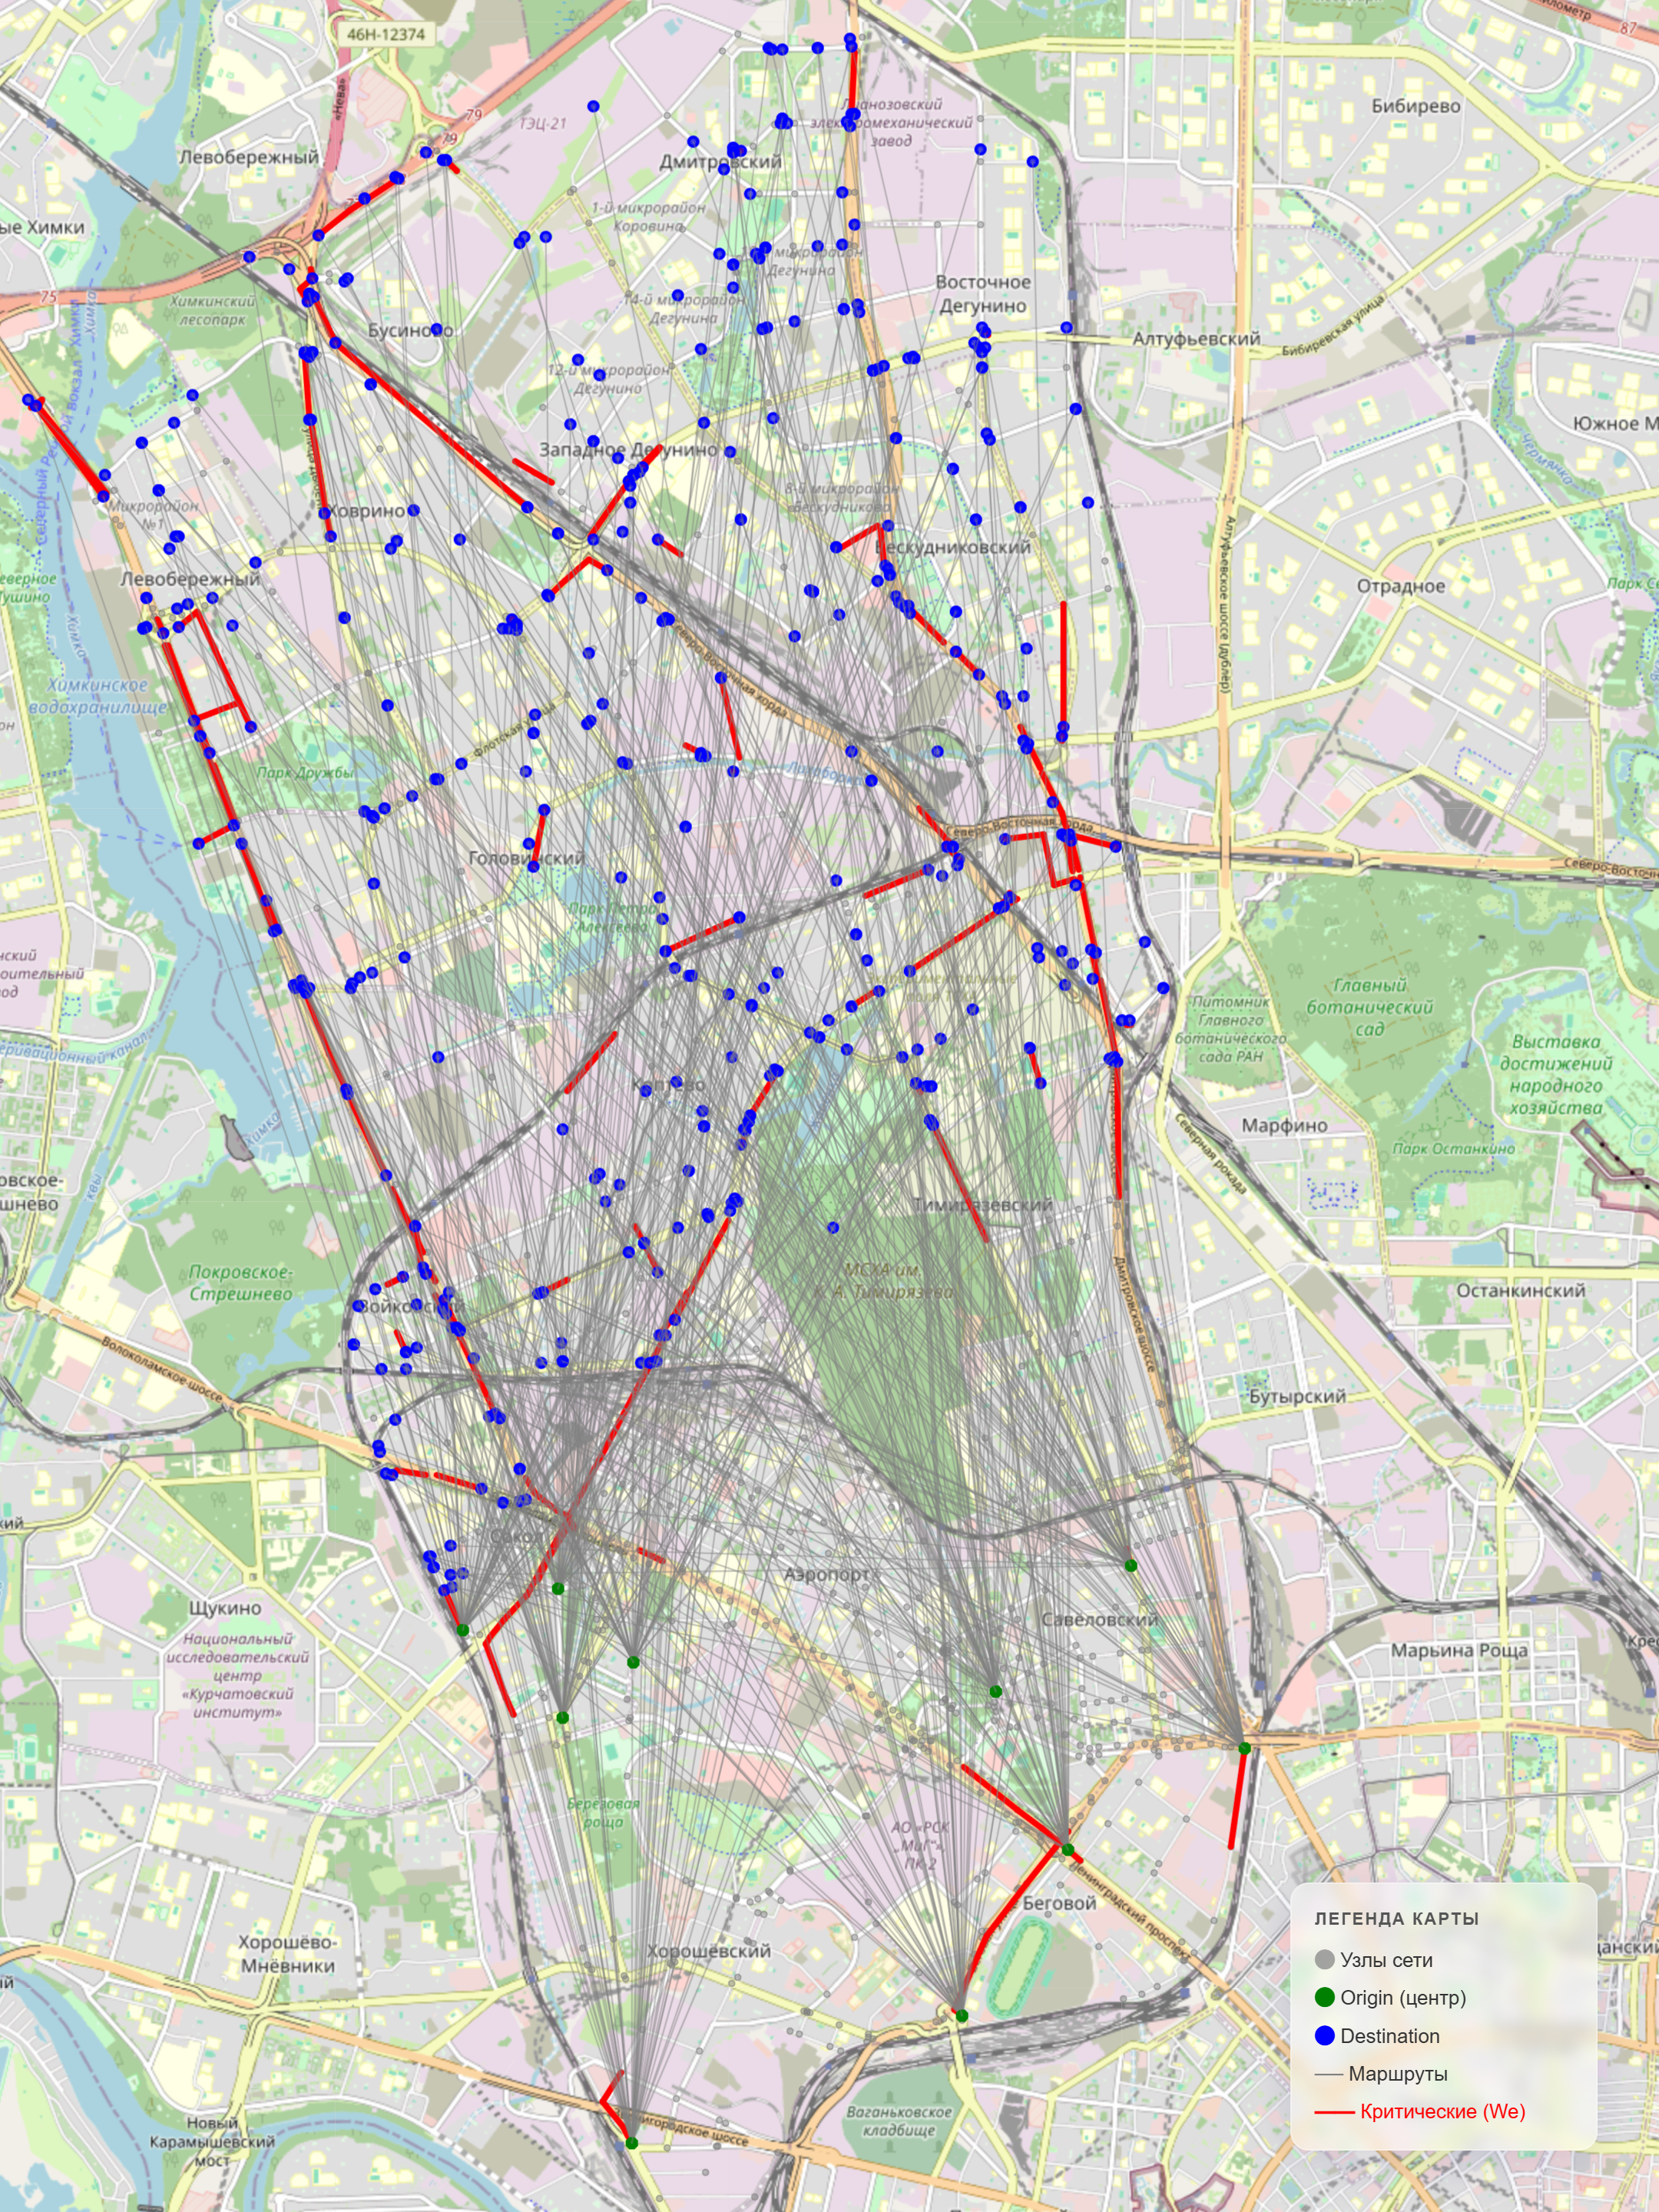
\includegraphics[width=\textwidth]{./view/SAO_3x4.png}
        \label{fig:sao_plot}
    \end{minipage}\hfill
    \begin{minipage}{0.32\textwidth}
        \centering
        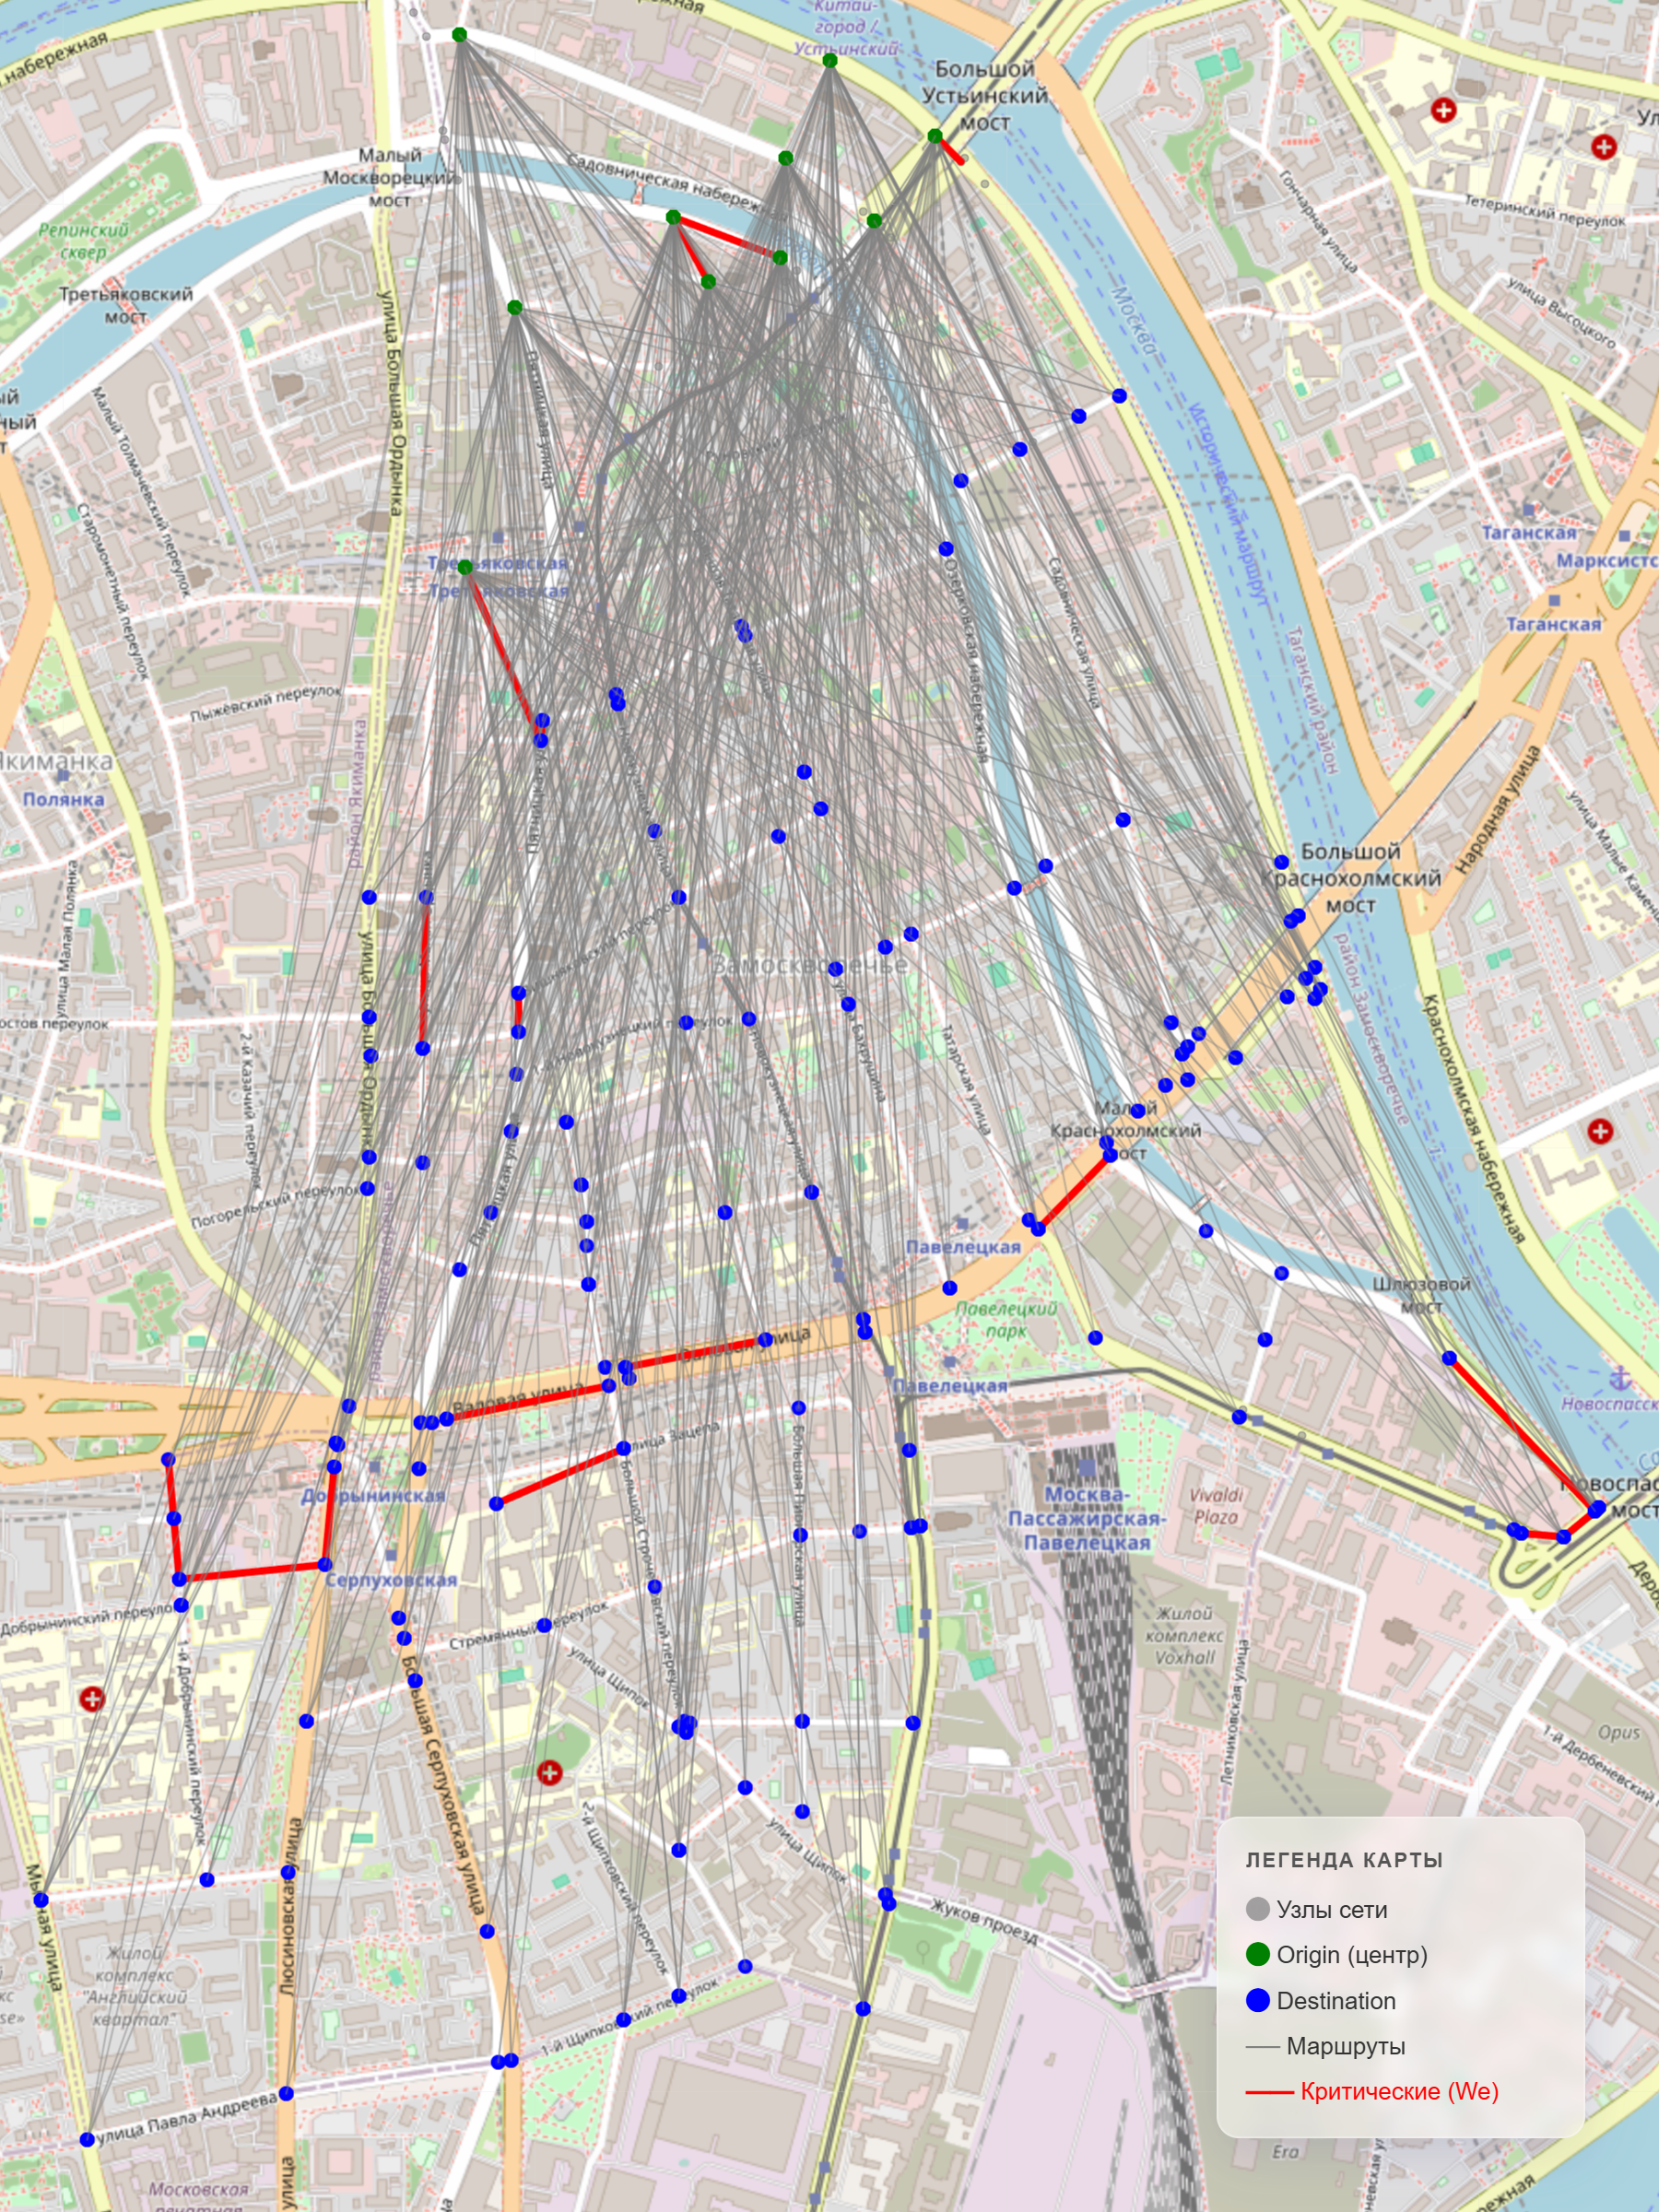
\includegraphics[width=\textwidth]{./view/ZMR_3x4.png}
        \label{fig:zmr_plot}
    \end{minipage}
    \begin{minipage}{0.32\textwidth}
        \centering
        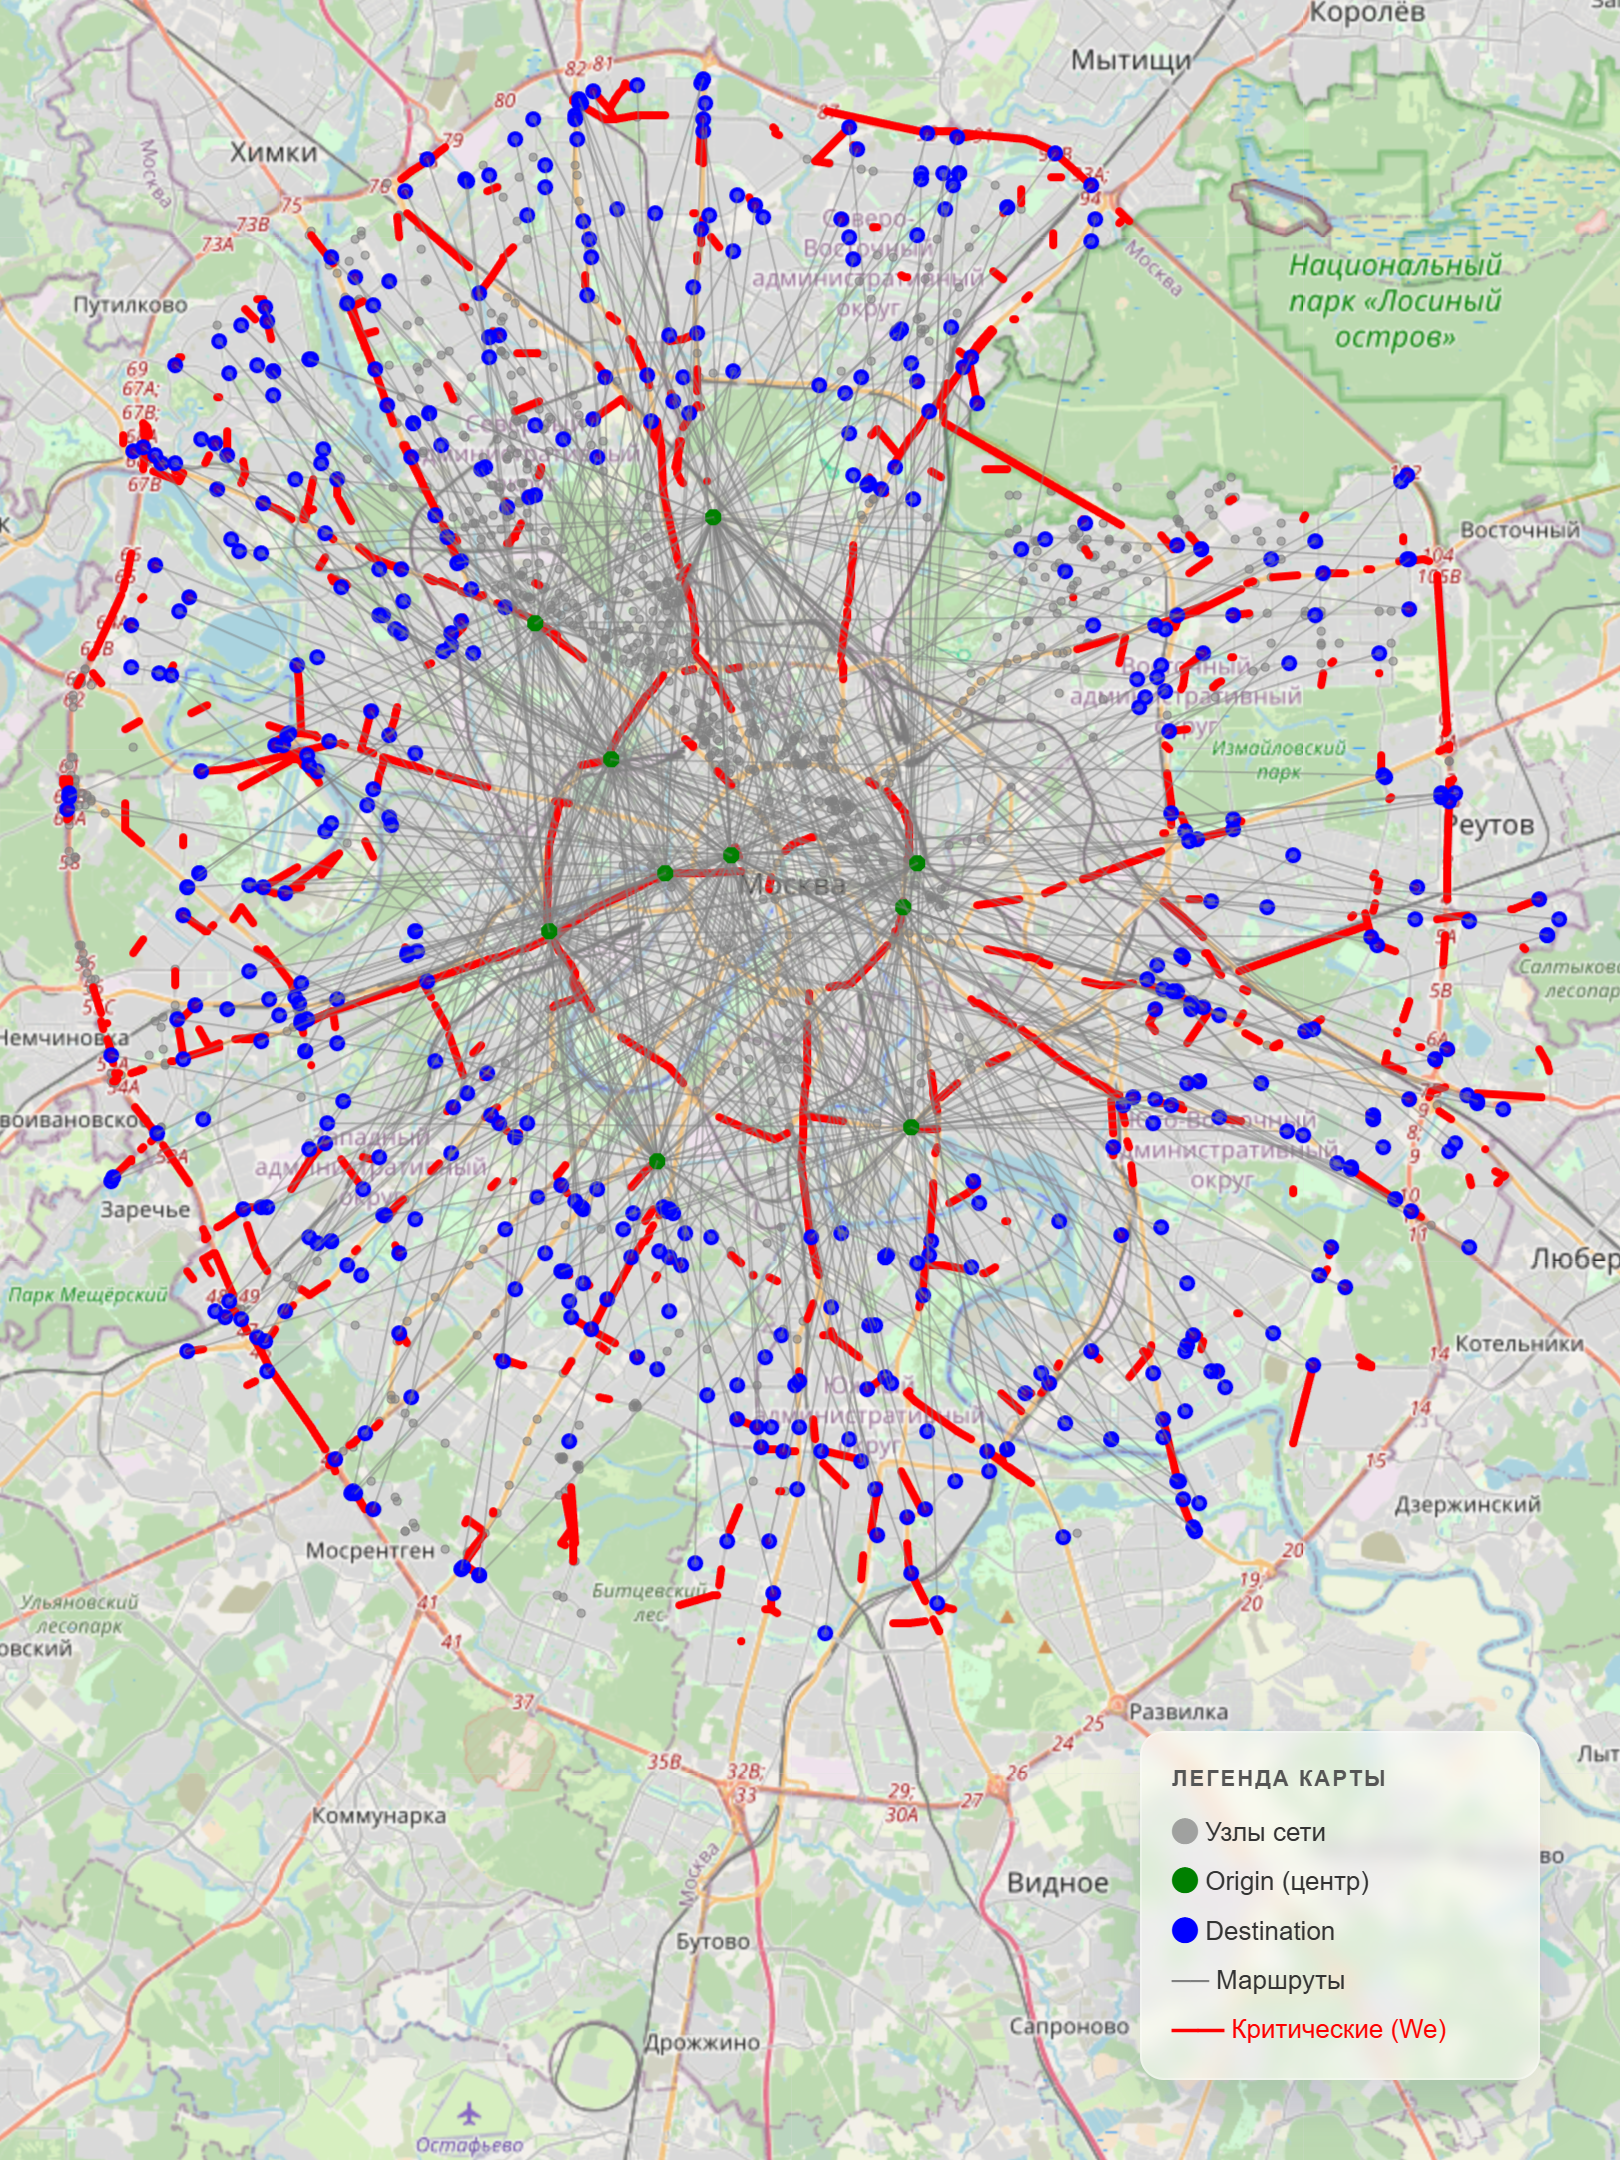
\includegraphics[width=\textwidth]{./view/MOSCOW_3x4.png}
        \label{fig:moscow_plot}
    \end{minipage}\hfill

    \caption{Графы транспортной сети: САО (слева), Замоскворечье (в центре), Москва (справа)}
    \label{fig:graphs_all}
\end{figure}


\begin{multicols}{2}

Наглядные геопространственные визуализации, выполненные с помощью Folium и Kepler.gl, 
позволили локализовать наиболее уязвимые участки на карте города и продемонстрировали, 
как именно распространяются заторы при превышении установленного порога (см. рис.~\ref{fig:graphs_all}). Полученные количественные данные подтверждают гипотезу о том, 
что для предотвращения масштабного транспортного коллапса критически важно не только учитывать топологию сети, но и динамику потоков, 
а также фокусировать внимание на защите и резервировании конкретных ключевых инфраструктурных элементов.

\section{Заключение}

Моделирование показало, что при случайном выведении элементов из строя сеть демонстрирует плавный переход от связной системы к хаотичной 
и сохраняет связность вплоть до удаления 42\% ребер. При этом моделирование целенаправленной атаки установило критический порог перколяции ($p_c=0.28$), 
при достижении которого потеря всего 28\% ключевых рёбер приводит к катастрофической фрагментации транспортной системы и потере ее функциональной связности. 
Полученные количественные данные и визуализации подтверждают необходимость учета динамических характеристик сети и 
фокусирования усилий на защите и резервировании конкретных уязвимых элементов инфраструктуры для предотвращения масштабных транспортных коллапсов.

\end{multicols}


\begin{thebibliography}{99}

\bibitem{rbc2025}
Десятибалльные пробки в Москве из‑за перекрытия центра 11 декабря 2025 года // РБК. 2025. URL: https://www.rbc.ru/society/11/12/2025/693ae9839a79476666be9d4c (дата обращения: 22.12.2025).

\bibitem{gluharuv1995}
Глухарёв К. К., Вишнев И. П., Исаков А. В., Фролов К. В. Устройство транспортной системы и способ регулирования транспортно‑пассажирским потоком мегаполиса: патент РФ №2104363. Заявл. 24.05.1995. Опубл. 10.05.1998.

\bibitem{gluharuv2013}
Глухарёв К. К., Валуев А. М., Калинин И. Н., Улюков Н. М. О моделировании автомобильных потоков на магистральной сети // Труды Московского физико‑технического института. 2013. Т. 5, № 4 (20). С. 102–114.

\bibitem{nekrasova2015}
Некрасова А. А., Соколов С. С. Исследование возможности применения теории перколяции для управления потоками данных в информационных сетях на транспорте // Сборник научных трудов Государственного университета морского и речного флота имени адмирала С. О. Макарова. 2015. № 35. С. 138–146.

\bibitem{khabarov2024}
Хабаров В. И., Беков М. А., Квашнин В. Е. Критические объекты транспортной инфраструктуры мегаполисов и агломераций // Вестник Сибирского государственного университета путей сообщения. 2024. № 3 (70). С. 20–27.

\bibitem{gasparyan2025}
Гаспарян Г. А. Обнаружение критически важных звеньев в пространственно‑временных маршрутных сетях с использованием теории сложных сетей // Crede Experto: транспорт, общество, образование, язык. 2025. № 3. С. 131–142.

\bibitem{pyatin2020}
Пятин Д. С. Совершенствование методов решения задачи автоматизированного планирования сети лесных дорог // Современные проблемы лесного хозяйства: материалы Всероссийской научно‑практической конференции. Санкт‑Петербург, 2020. С. 127–131.

\bibitem{katarov2023}
Катаров В. К., Рожин Д. В., Сюнёв В. С. Оптимальное проектирование сети лесных дорог: от методов к решениям // Resources and Technology. 2023. Т. 20, № 3. С. 32–47.

\bibitem{balamirzoev2019}
Баламирзоев А. Г., Батманов Э. З., Султанахмедов М. А., Муртузов М. М., Игитов Ш. М. Управление транспортными потоками на основе перколяционной стохастической модели // Информационные технологии в науке и образовании: материалы Всероссийской научно‑практической конференции. Махачкала: Алеф, 2019. С. 13–16.

\end{thebibliography}

\newpage
\pagestyle{empty}

\section{Приложение}

\begin{figure}[H]
    \centering
    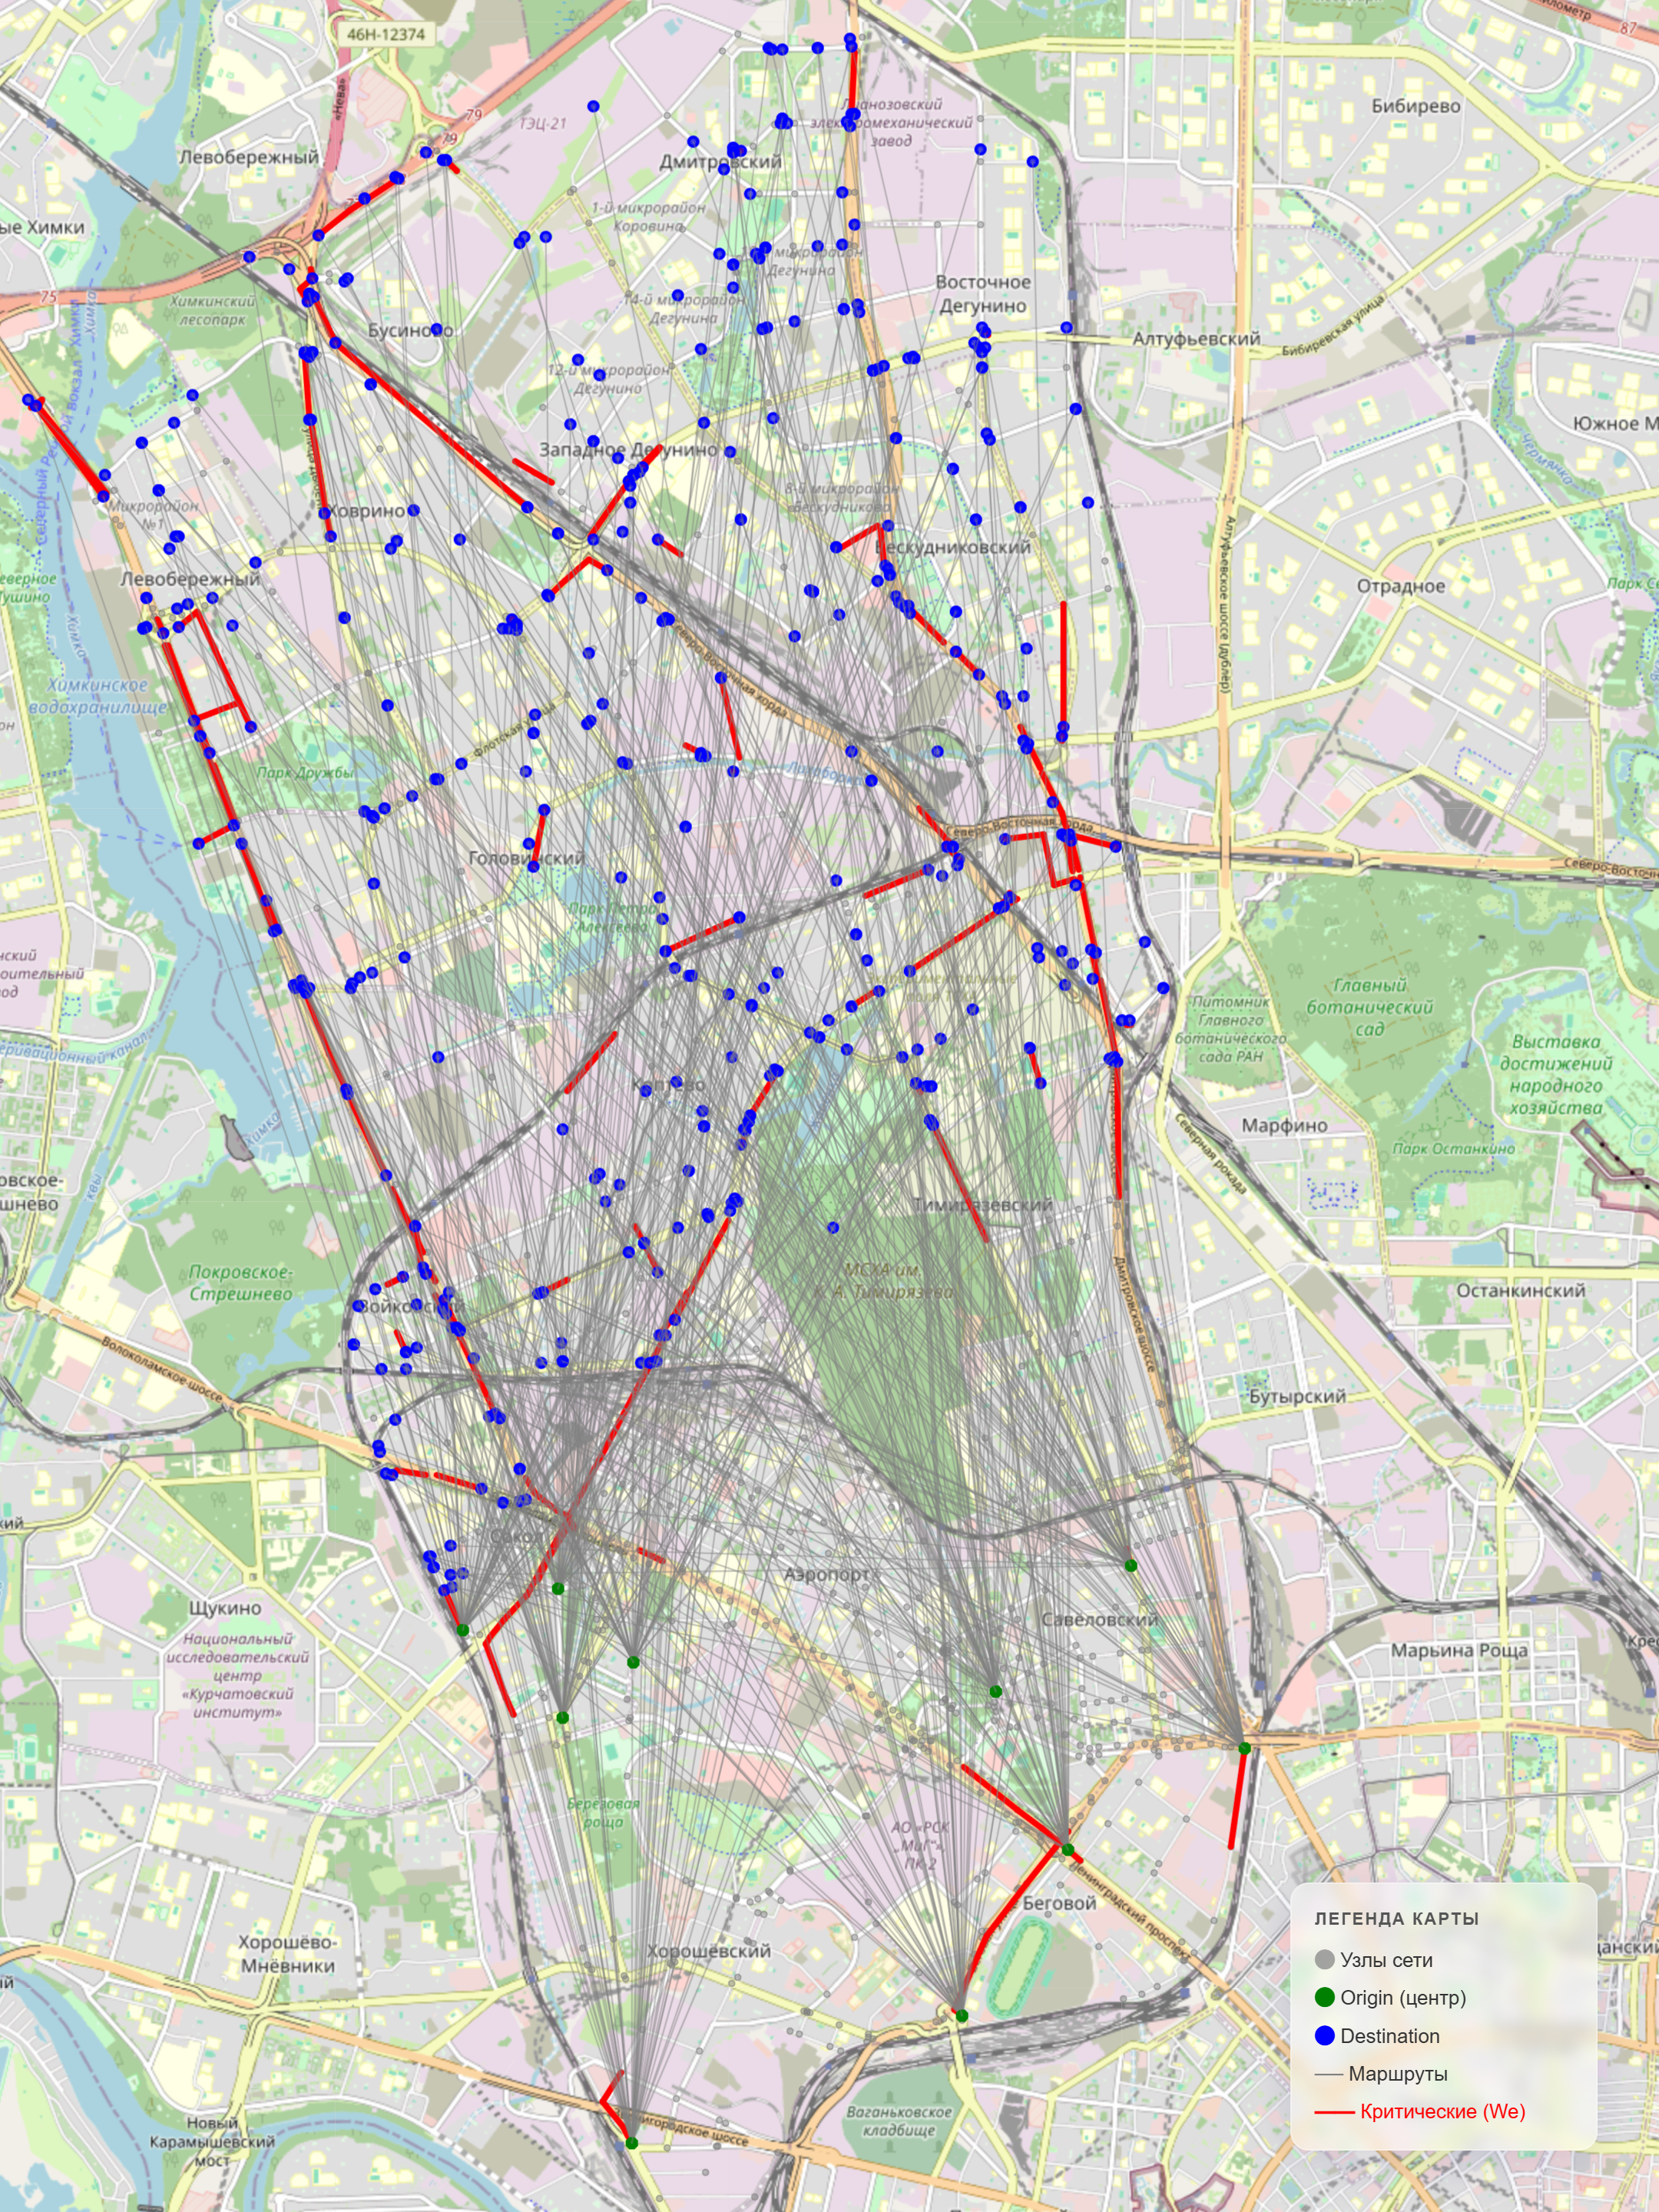
\includegraphics[width=\textwidth]{./view/SAO_3x4.png}
    \caption{Граф sao}
    \label{fig:p_sao_plot}
\end{figure}

\begin{figure}[H]
    \centering
    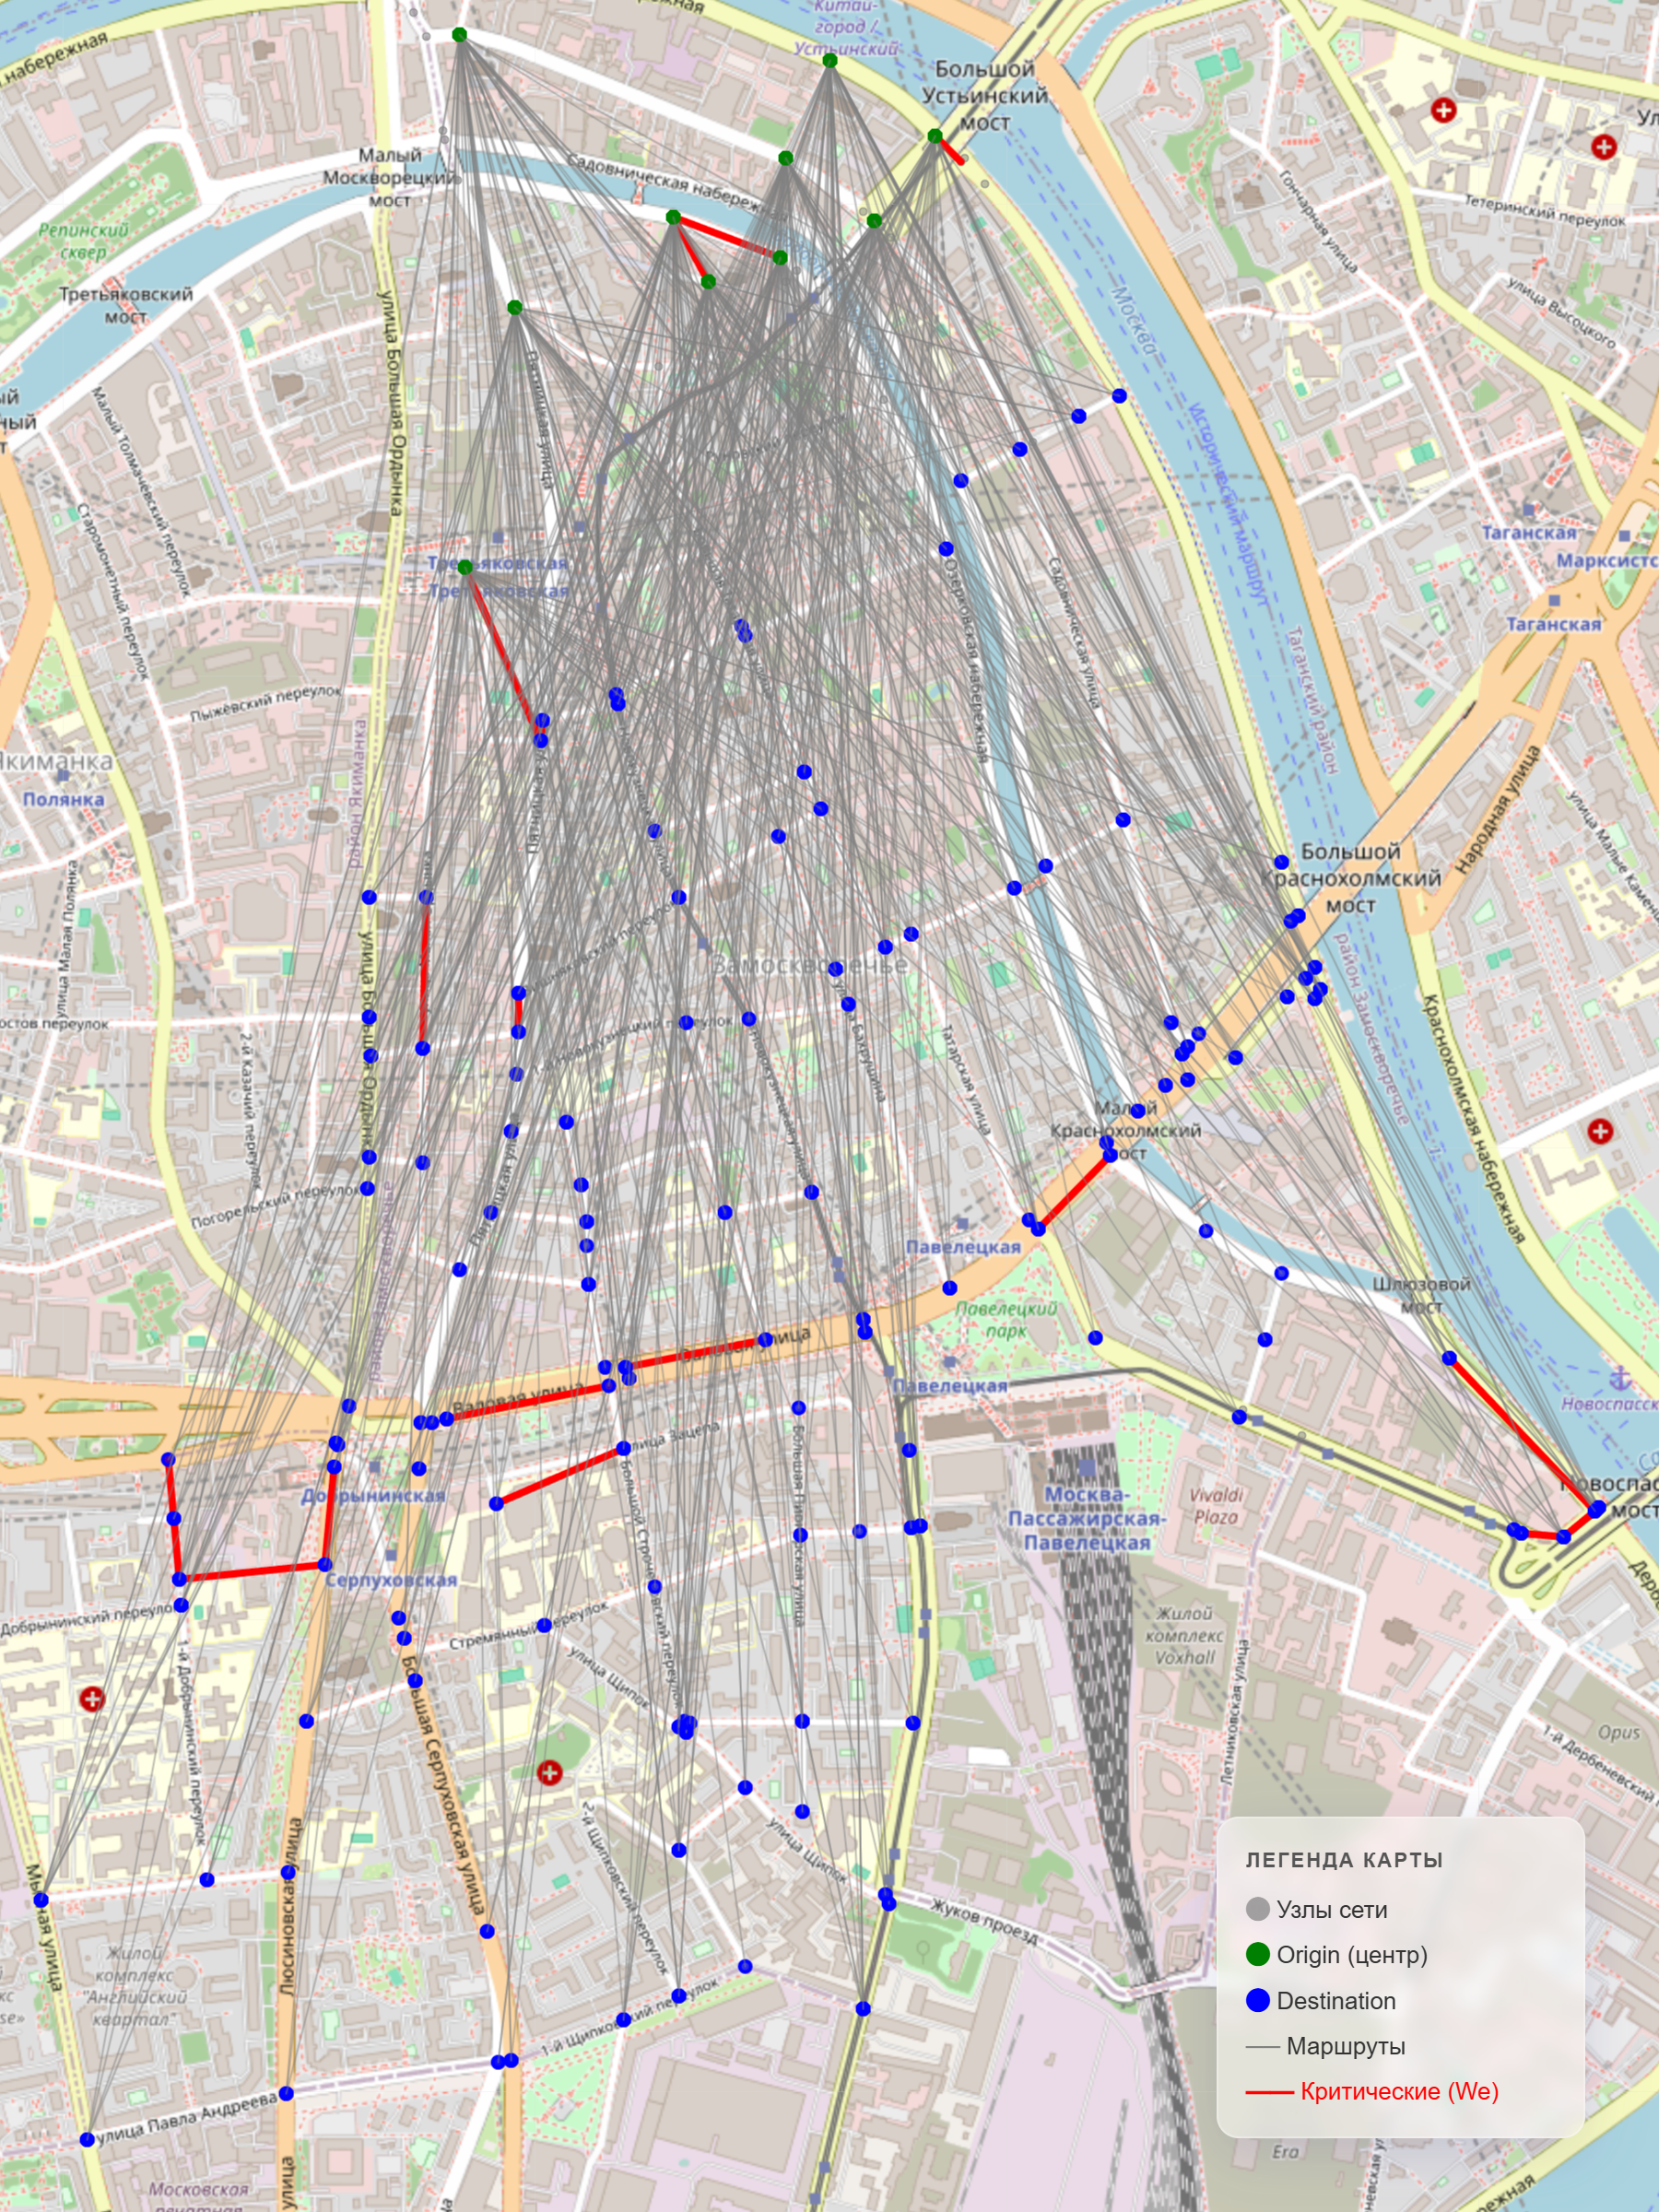
\includegraphics[width=\textwidth]{./view/ZMR_3x4.png}
    \caption{Граф zmr}
    \label{fig:p_zmr_plot}
\end{figure}

\begin{figure}[H]
    \centering
    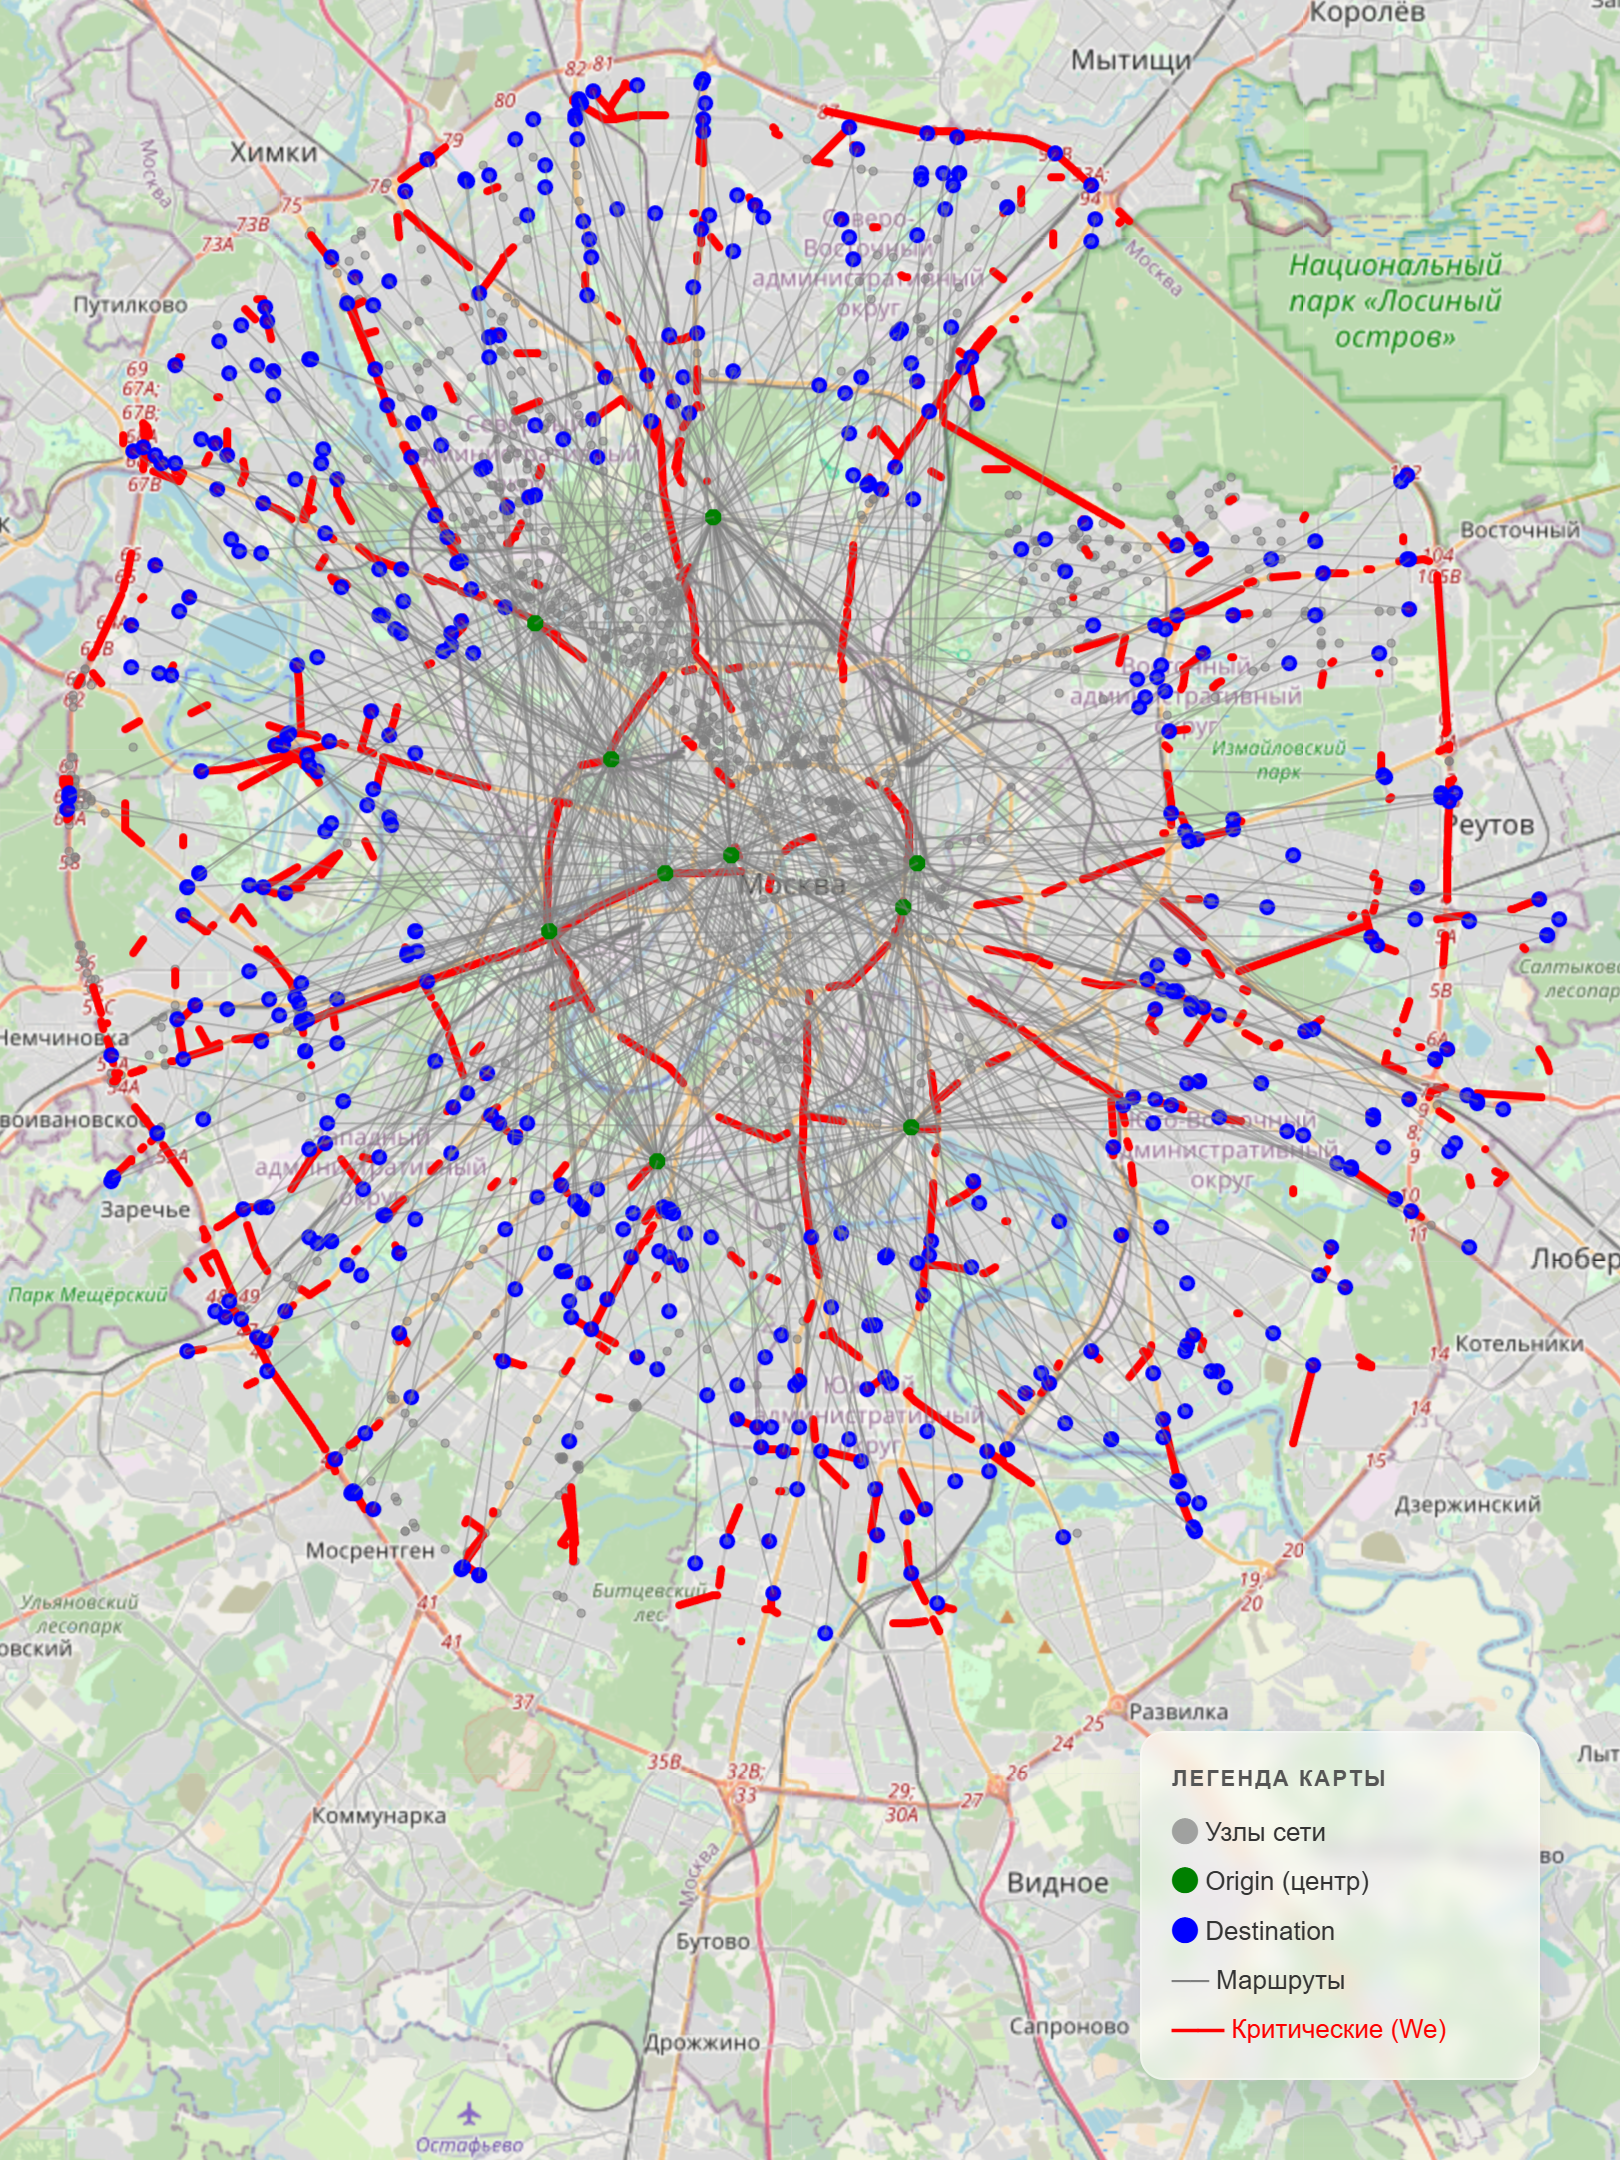
\includegraphics[width=\textwidth]{./view/MOSCOW_3x4.png}
    \caption{Граф moscow}
    \label{fig:p_moscow_plot}
\end{figure}

\begin{figure}[H]
    \centering
    \includegraphics[width=\textwidth]{./view/sao_plot.png}
    \caption{Перколяционный анализ для САО: зависимость LCC и Efficiency от доли удалённых рёбер}
    \label{fig:p_sao}
\end{figure}

\begin{figure}[H]
    \centering
    \includegraphics[width=\textwidth]{./view/zmr_plot.png}
    \caption{Перколяционный анализ для Замоскворечья: зависимость LCC и Efficiency от доли удалённых рёбер}
    \label{fig:p_zmr}
\end{figure}

\begin{figure}[H]
    \centering
    \includegraphics[width=\textwidth]{./view/moscow_plot.png}
    \caption{Перколяционный анализ для Москвы (5000 OD-пар): зависимость LCC и Efficiency от доли удалённых рёбер}
    \label{fig:p_moscow}
\end{figure}

\begin{figure}[H]
    \centering
    \includegraphics[width=\textwidth]{./view/moscow_1000_plot.png}
    \caption{Перколяционный анализ для Москвы (5000 OD-пар): зависимость LCC и Efficiency от доли удалённых рёбер}
    \label{fig:p_moscow_1000}
\end{figure}

\end{document}
